\subsubsection{Lavpasfilter} \label{sec:lavpas_test}
For at undersøge, hvilken betydning det digitalt filtrede signal har i forhold til det samplede signal, visualiseres dette. 
De samplede signaler er fra pilotforsøget, som er beskrevet i \autoref{sec:pilotforsoeg}. 
Signalerne sendes til mikrokontrollen via en UART-forbindelse, hvorved den filtrede værdi returners og visualisers i MATLAB. 
Dette fremgår af \autoref{fig:lavpas_imp}.

\begin{figure}[H]
\centering
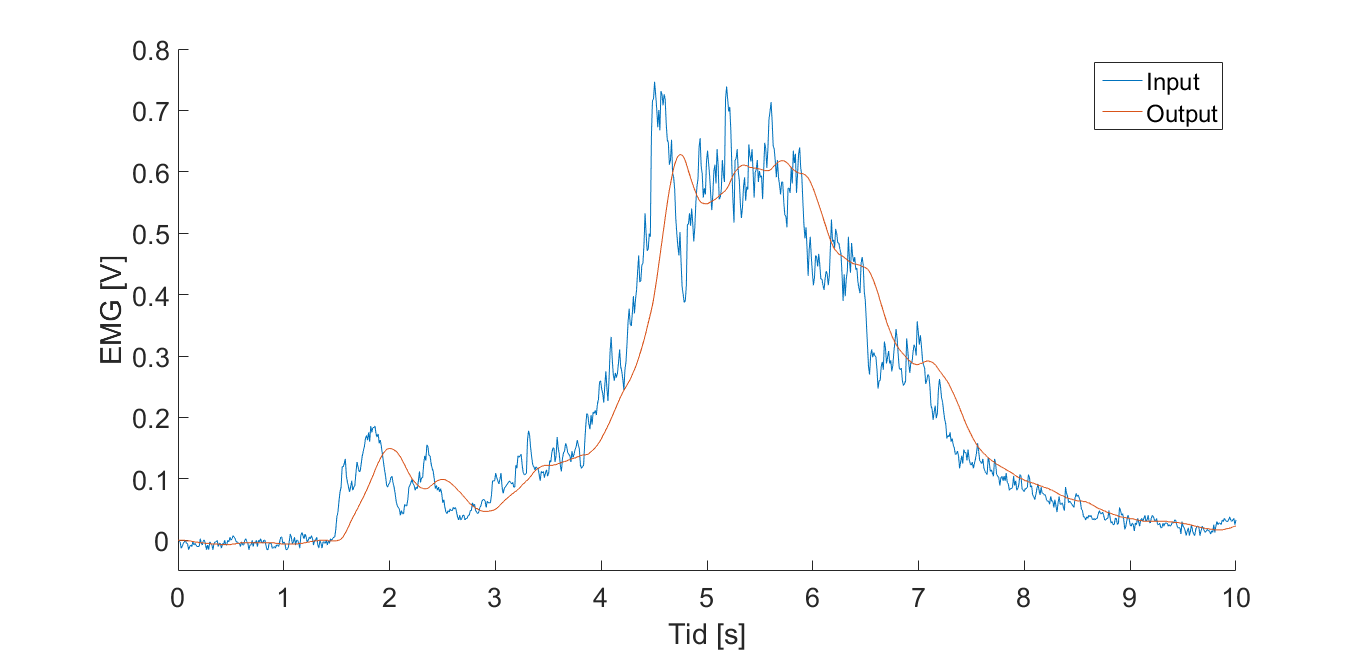
\includegraphics[width=1\textwidth]{figures/EMG_test}
\caption{Den blå graf illustrerer et samplet muskelsignal, og den røde graf illustrerer et samplet filtreret muskelsignal.}
\label{fig:lavpas_imp}
\end{figure}

\noindent
Figuren illustrerer, at inputsignalet følger det samplede signal dog med forsinkelse. 
For at teste forsinkelsen idet filtret eksekveres, defineres en debug-pin på mikrokontrolleren. Denne pin tillader tilslutning af eksterne instrumenter, således en eksekveringstid af koden kan måles.  
Denne pin defineres til at være høj før funktionskaldet og lav efter funktionskaldet. 
For at måle, hvor længe pin'en er høj, tilsluttes et oscilloskop. 
Ud fra dette aflæses en forsinkelse på $175~\mu s$, hvilket er tiden det tager for data at passere det digitale filter.
Denne forsinkelse vurderes ikke at have nogen signifikant betydning i forhold til det samlede system.

For at vurdere om filteret dæmper nok i forhold til de opstillede krav i \autoref{sec:lavpas_krav}, udføres en test, hvor forskellige frekvenser sendes gennem filteret. 
Hertil anvendes en funktionsgenerator til at generere et signussignal mellem $0,5-20~Hz$. 
Disse frekvenser er valgt for at teste dæmpningen i pasbåndet og i transitionsbåndet.  
%Dette frekvensområde er valgt på baggrund af målinger fra \autoref{sec:pilotforsoeg}, hvor det fremgår, at signalet ligger mellem $0,4-10~Hz$.  
%Da funktionsgeneratoren ikke kan indstilles til en frekvens på $0~Hz$ indstilles denne til $1~\mu~Hz$. 
Amplituden af sinussignalet sættes til $1~V_{pp}$ med et offset på $1,65~V$, da dette fortages ved single ended måling, hvortil sinussignalet ikke kan svinge omkring $0~V$. 
Yderligere tilsluttes et oscilloskop til funktionsgeneratoren for at kontrollere det genererede signal. Af oscilloskopet aflæses amplituden til $1,08~V$.  
For at omregne det konverterede filtrerede signal til en spænding, ganges de samplede værdier med LSB for ADC'en. 
Da amplituden for inputsignalet og det filtrerede signal kendes, anvendes \autoref{eq:deampning_dB} til at udregne en dæmpning i dB.

\begin{equation} \label{eq:deampning_dB}
	dB = 20 \cdot log_{10}(\frac{V_{in}}{V_{out}})
\end{equation}

\noindent
Dæmpningen ved de forskellige frekvenser fremgår af \autoref{fig:bodeplot}.

\begin{figure}[H]
\centering
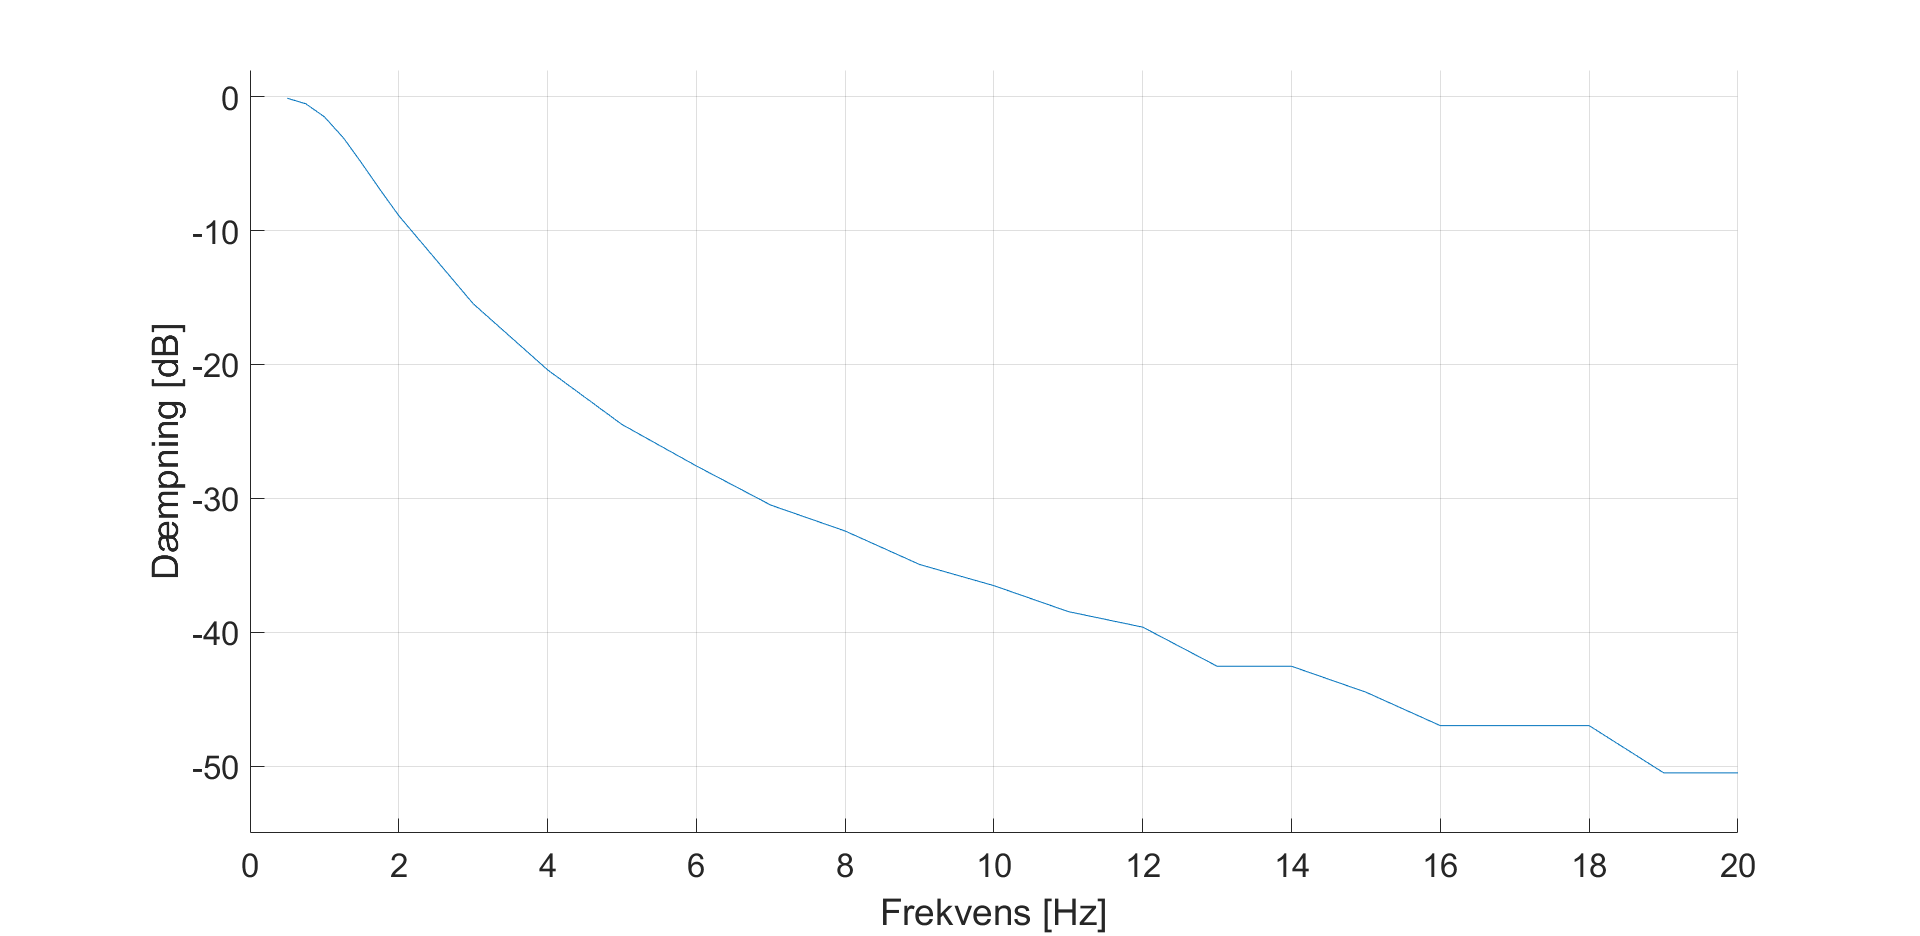
\includegraphics[width=1\textwidth]{figures/bodeplot_lavpas2}
\caption{Bodeplot for lavpasfiltret. Heraf fremgår dæmpningen ved forskellige frekvenser idet de passerer lavpasfiltret.}
\label{fig:bodeplot}
\end{figure}

\noindent
Yderligere testes dæmpningen for knækfrekvensen, der forventes at være $3~dB$. 
Resultatet heraf viser en dæmpning på $3,1~dB$ ved en frekvens på $1,26~Hz$. 
Dette stemmer overens med et Butterworthfilter, hvortil afvigelsen på $0,1~dB$ ikke antages som værende af signifikant betydning i forhold til systemets virkemåde. 
På baggrund af de udførte tests godtages filtret. 

%\noindent
%En dæmpning på $-3~dB$ for den valgte knækfrekvens på $1,26~Hz$ bestemmes, samt en dekade længere ude svarende til en frekvens på $50~Hz$. Da der anvendes et 2. ordens filter, skal denne frekvens dæmpes ved $-40~dB$. Da der er anvendt EMG-forstærkeren fremgår $50~Hz$ ikke, hvilket er beskrevet i \autoref{sec:EMG_imp}. Outputspændingen ved dennee dæmpningsfaktor er udregnet ved \autoref{equ:daempning1}. 
%
%\begin{equation} \label{equ:daempning1}
%-3~dB = 20 \cdot log_{10} \cdot (\frac{V_{out}}{1}) \Rightarrow V_{out} = 0,7 V
%\end{equation}
%
%\noindent
%Da det ikke er muligt at aflæse nøjagtige værdier for Vpp tages der udgangspunkt i de nærmeste værdi. Værdien for $1,26~Hz$ er  aflæst til $0,06~V$. Afvigelsen fremgår af \autoref{equ:afvigelse1}.
%%Da målingerne for $V_{pp}$ ikke er muligt at aflæse nøjagtige værdier, hvorfor der tages udgangspunkt i de nærmeste værdier. Værdierne for $5~Hz$ er $0,06~V$. Afvigelsen fremgår af \autoref{equ:afvigelse1}.
%
%\begin{equation} \label{equ:afvigelse1}
%Afviglese_{5~Hz} = \frac{0,06V-0,7V}{0,7V} \cdot 100\%  = - 14 \%
%\end{equation}
%
%\noindent 
%Afvigelserne for $1,26~Hz$ er 14\%. Dette betyder at filteret ikke dæmper signalet nok. Da målingerne for outputspændingen, målt ved de forskellige frekvenser, ikke er nøjagtig aflæst er det forventet, at der er en større afvigelse fra værdierne udregnet i \autoref{equ:daempning1}. På baggrund af dette godtages filteret. 

\vspace{3mm}
\textbf{Opsummering af krav:}
\begin{itemize}
\item[\text{\sffamily \checkmark}] Skal følge inputsignalet mest muligt  
\item[\text{\sffamily \checkmark}] Skal udformes som et Butterworth lavpasfilter
\item[\text{\sffamily \checkmark}] Skal have en knækfrekvens på $1,26~Hz$
\item[\text{\sffamily \checkmark}] Skal have en filterorden på 2
\end{itemize}